\documentclass[a4paper,11pt]{article}
\usepackage[utf8]{inputenc}
\usepackage[paper=a4paper, hmargin=1.5cm, bottom=1.5cm, top=3.5cm]{geometry}
\usepackage[T1]{fontenc}
\usepackage[spanish]{babel}
\usepackage[colorlinks=true, linkcolor=blue]{hyperref} %Links para el indice.

\usepackage{amsfonts}
\usepackage{graphicx}
\usepackage{verbatim}
\usepackage{listings}
\usepackage{algorithm}
\usepackage{algpseudocode}
\usepackage{graphicx}

\newcommand{\real}{\hbox{\bf R}}

\title{Trabajo Práctico de Métodos Númericos}
\author{Castro, Dami\'an \& Matayoshi, Leandro \& Szyrej,Alexander}

\begin{document}
\begin{center}
	Universidad de Buenos Aires - Departamento de Computaci\'on - FCEN
\end{center}

\rule{\linewidth}{0.5mm}

\vspace{1cm}

\begin{center}
	\Huge{Trabajo Práctico de Métodos Númericos}
\end{center}


\vspace{4cm}


Integrantes:
\begin{itemize}
	\item Castro, Dami\'an L.U.: 326/11  \verb+ltdicai@gmail.com+
	\item Matayoshi, Leandro L.U.: 79/11 \verb+leandro.matayoshi@gmail.com+
	\item Szyrej, Alexander L.U.: 642/11   \verb+alexanderszyrej@gmail.com+
	
\end{itemize}


%\maketitle

\vspace{4cm}

Palabras Clave:
\begin{itemize}
	\item Ra\'ices Reales
	\item Newton-Raphson
	\item Convergencia de m\'etodos iterativos
\end{itemize}


\newpage

\tableofcontents

\newpage

\section{Introducción teórica}

Durante el desarrollo de la mayoría de los proyectos en programación, como es el caso de la implementación de videojuegos como el Quake III, deben realizarse sucesivas operaciones matematicas para, por ejemplo, normalizar vectores o trabajar con diversas variables matemáticas. Así mismo, es de 
suma importancia que estas operaciones se realicen en tiempo y forma, es decir, rápido y bien. Para ello, en ocasiones uno prefiere dejar de lado el uso de la FPU para en cambio utilizar métodos númericos que, luego de sucesivas iteraciones, alcancen una aproximación del valor deseado que se considere suficientemente precisa más rápidamente. Esta preferencia por los métodos iterativos termina acelerando todo el proyecto a largo plazo puesto que suelen ser muy numerosas las operaciones a realizar y muy costosas de hacer de forma exacta en la FPU.

~

En este trabajo práctico analizaremos cuatro de estos métodos para el cálculo de la raiz cuadrada de un número real positivo ($\alpha$): 
\begin{itemize}
	\item Newton-Raphson.
	\item Bisección.
	\item Secante.
	\item Regula Falsi.
\end{itemize}

Estos se denominan métodos iterativos de punto fijo \footnote{http://math.fullerton.edu/mathews/n2003/FixedPointMod.html para más información, y unas animaciones didácticas: http://math.fullerton.edu/mathews/a2001/Animations/RootFinding/FixedPoint/FixedPoint.html} y a grandes rasgos, para hallar la raíz de una función $f(x)$ encuentran el punto fijo $p$ de una función auxiliar $g(x)$ (es decir, $g(p) = p$) de manera tal que $f(p) = 0$. 

En particular los usaremos para hallar las raíces de dos funciones a conocer:

\begin{itemize}
	\item $f(x) = x^2 - \alpha$
	\item $\displaystyle e(x) = \frac{1}{x^2} - \alpha$
\end{itemize}

Notar que hallar la raíz de $f(x)$ equivale a calcular el valor de $\sqrt{\alpha}$, así como para $e(x)$ hallamos el valor de $\displaystyle 
\frac{1}{\sqrt{\alpha}}$.

\subsection{Breve descripción de los métodos}

En general, los cuatro métodos son similares entre sí dado que todos ellos generan una sucesión de puntos que, en el mejor de los casos, tiende al valor que estamos buscando, es decir, converge a la raiz de la función. Sino decimos que el método diverge, y esto por lo general depende del valor inicial que tomemos (semilla). Es la rapidez con la que alcanzan dicho valor lo que los diferencia.

%Se entiende por convergencia de un método numérico la garantía de que, al realizar un buen número de repeticiones (iteraciones), las aproximaciones obtenidas terminan por acercarse cada vez más al verdadero valor buscado.

%En la medida en la que un método numérico requiera de un menor número de iteracciones que otro, para acercarse al valor numérico deseado, se dice que tiene una mayor rapidez de convergencia.

~

Newton-Raphson \footnote{http://nm.mathforcollege.com/topics/newton$\_$raphson.html} es un algoritmo eficiente para el problema de cero de funciones. Dado que converge cuadráticamente bajo ciertas hipótesis analizaremos exhaustivamente éste método implementado sobre ambas funciones. Luego decidiremos que métodos alternativos se pueden utilizar para cada función, dado que los restantes son más sencillos a nivel implementación pero su convergencia no es tan buena en comparación con el método de Newton, i.e. se aproximan más lentamente a la solución esperada.

Bisección \footnote{http://nm.mathforcollege.com/topics/bisection$\_$method.html} por ejemplo posee una convergencia lineal, pero su utilidad recae en que siempre converge, aún con semillas (valores iniciales) muy alejadas del valor a encontrar, y es por esto que lo analizaremos no sólo como método alternativo sino también como generador de semillas para los demás métodos.

Por otro lado, tanto Secante como Regula Falsi superan a Bisección en convergencia, pero no alcanzan a Newton (convergencia superlineal). Su problema recae en las hipótesis de convergencia. Más adelante veremos su desempeño en comparación con los métodos ya mencionados. 
\footnote{http://nm.mathforcollege.com/topics/secant$\_$method.html $\&$ http://nm.mathforcollege.com/topics/false$\_$position.html}

~

A continuación, una detallada descripción del desarrollo del presente trabajo.


\section{Desarrollo}

Como habíamos mencionado anteriormente, el objetivo del trabajo es encontrar las raíces de $f(x)=x^{2} - \alpha$ y $e(x) = 1/x^{2} - \alpha$.
Para resolver el problema, implementamos para ambas funciones los cuatro métodos iterativos vistos en clase : Bisección, Newton, Regula Falsi y Secante.
La explicación y la base teórica de los mismos puede ser encontrada fácilmente en distintos libros de métodos numéricos, como
por ejemplo: "Numerical Analysis, Burden \& Faires". 

\subsection{Estructura del código}

Antes de comenzar a escribir código decidimos realizar una breve etapa de diseño, en donde nos propusimos encapsular algunos comportamientos para poder escribir un programa
más prolijo y legible.

Lo primero que hicimos fue diseñar una clase llamada $Funciones$. La idea es la siguiente: sea $h$ la función que estamos analizando (podría ser tanto $f$ como $e$).
Como los métodos requieren evaluar $h$ para calcular el valor de la sucesión en los términos siguientes (y algunos $h\_derivada$), sería bueno encapsular estos cálculos
con un comportamiento similar al de una ''caja negra'' (la famosa caja negra). Esto es: en lugar de efectuar la operación en el scope de la función que ejecuta el método,
invocamos a $Funciones.h(x)$ o $Funciones.h\_derivada(x)$, desligándonos de la forma en que estas están implementadas.

Esto es particularmente notorio y beneficioso, por ejemplo, para el código de Newton\_e (i.e: método de Newton para la función $e$. De ahora en más utilizarmos esta notación
para referirnos a los distintos algoritmos):

$\displaystyle e\_deriv = \frac{-2}{x^{3}} \Rightarrow x_{n+1} = x_{n} - \frac{\frac{1}{x_{n}^2}-\alpha}{\frac{-2}{x_{n}^{3}}} \Rightarrow 
x_{n+1} = x_{n} + \frac{(x_{n} - \alpha x_{n}^{3})}{2} $ 

Newton\_e encapsula todos esos cálculos mediante las operaciones:

~

$x_{n+1} = x_{n} - \frac{Funciones.e(x_{n})}{Funciones.e\_deriv(x_{n})}$

~

Luego, por razones muy similares a la anterior, decidimos abstarer el funcionamiento de los criterios de parada, mediante una clase llamada $Criterios$. La decisión de
''cuándo parar'' es independiente al algoritmo que está siendo ejecutado. Además, eventualmente queremos evaluar el comportamiento de un mismo método con distintos 
criterios. Tomemos como ejemplo Bisección. Si hubiéramos implementado esa parte dentro del código del método, entonces habríamos tenido algo de este estilo:

~

\begin{algorithmic}
\Function{Biseccion}{seeds $positivo,negativo$}
	\State \ldots
	\While{$!(max\_iteraciones < i \lor |medio_i < medio_{i-1}| < \epsilon| \lor \frac{|medio_i < medio_{i-1}|}{|medio_{i-1}|} < \epsilon \ldots)}$ 
		\State $\displaystyle medio_{i-1} = medio$
		\State $\displaystyle medio_{i} = \frac{positivo_{i}+negativo_{i}}{2}$
		\State \ldots
	\EndWhile
\EndFunction
\end{algorithmic}

~

Por el contrario, utilizando la case tenemos:

\begin{algorithmic}
	\While{$!criterios.parar(parameters)$}
		\State \ldots
	\EndWhile
\end{algorithmic}

~

La existencia de class Criterios permite agrupar todo el código que esté relacionado con ellos en un solo bloque, con lo cual ahorramos tener que escribirlos
en cada una de las guardas del while de los distintos algoritmos. Al mismo tiempo resalta el aspecto independiente mencionado más arriba: Los criterios de parada son 
independientes a los métodos que los utilizan.





\section{Resultados}

% % \begin{figure}
% % 	\centering
% 	\begin{minipage}{.5\textwidth}
% 		\centering
% 		\includegraphics[keepaspectratio]{Imagenes/exp1/biseccion_f.pdf}
% 		\captionof{figure}{A figure}
% 		\label{fig:test1}
% 	\end{minipage}%
% 	\begin{minipage}{.5\textwidth}
% 		\centering
% 		\includegraphics[keepaspectratio]{Imagenes/exp1/biseccion_f.pdf}
% 		\captionof{figure}{Another figure}
% 		\label{fig:test2}
% 	\end{minipage}
% \end{figure}

\subsection{Primeras experimentaciones}

\begin{figure}[!h]
	\begin{center}
		  \includegraphics[keepaspectratio]{../Imagenes/exp1/biseccion_f.pdf}
		  \caption{Bisección\_f para $\alpha=4.0, \epsilon = 10^{-6}, criterio = 1\  con \ max\_iter=20$}
		  \label{fig:contra1}
	\end{center}
\end{figure}
\FloatBarrier
~

\begin{figure}[!h]
	\begin{center}
		  \includegraphics[keepaspectratio]{../Imagenes/exp1/biseccion_e.pdf}
		  \caption{Bisección\_e para $\alpha=6.0, \epsilon = 10^{-6}, criterio = 3$}
		  \label{fig:contra1}
	\end{center}
\end{figure}
\FloatBarrier
Los resultados tanto para $biseccion\_f$ como para $biseccion\_e$ fueron los esperados. Los métodos convergen al resultado para cualquier valor de $\alpha$ (Fueron evaluados valores entre 0 y 10000 aproximadamente,
con bastante granularidad). Para realizar los gráficos fueron elegidos los valores de $\alpha$ 4.0 para $f$ y 6.0 para $e$ únicamente debido a que permiten utilizar una escala que nos deja apreciar los aspectos
relevantes del análisis. Los puntos rojos corresponden al valor de $x$ en cada iteración del método. Con el correr de las iteradas, los puntos van amontonándose alrededor de la raíz teórica de la función.

Un aspecto llamativo de los resultados obtenidos en esta etapa es el hecho de que 
a medida que los valores de $\alpha$ crecen, bisección\_e requiere de una mayor cantidad de iteraciones (en comparación con $f$) para obtener un valor cercano a la raíz de la función. Por ejemplo,
tomando 40 iteraciones en cada experimento y variando el valor de alfa, obtuvimos que: 

Para $\alpha = 0.1$, $f(x\_40) \approx 1*10^{-13}$ y $e(x\_40) \approx 1*10^{-13}$. 

Para $\alpha = 7.0$ : 
$f(x\_40) \approx 1*10^{-11}$ y $e(x\_40) \approx 1*10^{-10}$. 

Y ya para $\alpha = 10000.0$: $f(x\_40) \approx 1*10^{-5}$ y $e(x\_40) \approx 0.01$

Notemos que estamos utilizando el criterio (3) para analizar la calidad de la solución obtenida.

Por lo general biseccion\_e se comprta peor que biseccion\_f (Terminar de pensar por qué)

Contrariamente a lo que suponíamos, al analizar newton\_f \ descubrimos que, luego de fijar $\alpha$ (distinto de cero), el método converge para cualquier semilla inicial que tomemos (también distinta de 0).
Pensemos un poco por qué sucede esto: 
Anteriormente ya demostramos que si $seed\_inicial > \sqrt{\alpha}$ entonces el método converge (ejercicio 3 de la práctica). 
Sin embargo, ¿ qué sucede cuando pertenece al itervalo $(0,\sqrt{\alpha})$. $x_1$ es el valor 
obtenido a partir de la interesección entre la recta tangente a $f(x)$ en $(x_0,f(x_0)$ y el eje de abscisas. Experimentalmente parecería ser que el valor de $x_1$ obtenido luego de la primera 
iteración es mayor a $\sqrt{\alpha}$. Este hecho puede explicarse en función la pendiente de la recta tangente en la semilla inicial. Como la misma tiene un valor peque\~no en módulo pero positivo
(menor a $2*\sqrt{\alpha}$), no es ilógico pensar que cortará al eje de abscisas en un valor de $x$ mayor a  $\sqrt{\alpha}$. El siguiente gráfico intenta representar esta idea:  

\begin{figure}[!h]
	\begin{center}
		  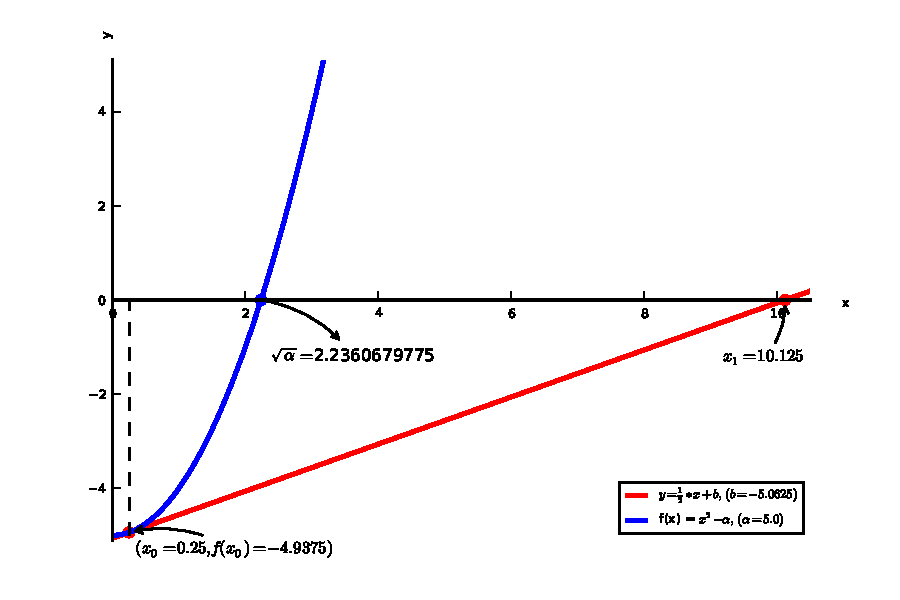
\includegraphics[keepaspectratio]{../Imagenes/exp1/recta_tangente.pdf}
		  \caption{Recta tangente a la curva con $x_0=0.25$ y $\alpha=5.0$}
		  \label{fig:contra1}
	\end{center}
\end{figure}
\FloatBarrier

Nótese que en los casos en donde $x_0$ comienza con valores peque\~nos en módulo obtenemos a partir de la primera iteración un $x\_1 >> \sqrt{\alpha}$. A medida que nos fuimos
acercando por izquierda, para valores en donde $x_{0} \approx \sqrt{\alpha}$,
experimentalmente también obtuvimos que $x\_1 > \sqrt{\alpha}$, lo cual explica el hecho de que newton\_f converja para cualquier semilla inicial.

En el siguiente gráfico mostramos un ejemplo de convergencia de newton\_f. Observemos que, a diferencia de bisección, el método converge luego de unas pocas iteraciones: ya no se 
produceese amontonamiento de puntos alrededor de la raíz teórica, a pesar de usar un epsilon 3 órdenes de magnitud más peque\~no 

\begin{figure}[!h]
	\begin{center}
		  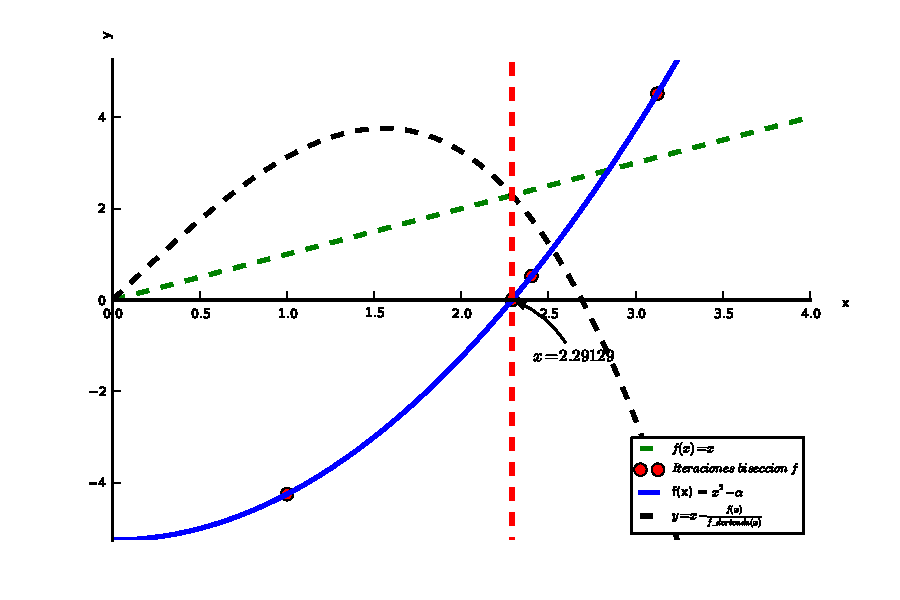
\includegraphics[keepaspectratio]{../Imagenes/exp1/newton_f.pdf}
		  \caption{newton\_f para $\alpha=5.25, \epsilon=10^{-8}, \ criterio = 5, \ seed = 1.0$}
		  \label{fig:contra1}
	\end{center}
\end{figure}
\FloatBarrier

En esta figura podemos apreciar por primera vez el comportamiento de una sucesión de punto fijo: el valor $c$ tal que $g(c)=c$ (donde $g(x) = x - \displaystyle \frac{f(x)}{f'(x)}$) es al mismo tiempo
raíz de la función $f$

Los resultados para Newton\_e, por el contrario, resultaron ser bastante distintos. Al evaluar el método para distintos valores de $\alpha$, descubrimos que: si la semilla inicial está comprendida en el intervalo
$(0,\frac{1}{\sqrt{\alpha}}]$ el método converge sin problemas. Sin embargo, empíricamente llegamos a la conclusión de que existe un $x_0$, con $x_0 > \frac{1}{\sqrt{\alpha}}$, tal que $\forall x \geq x_0$, el método
diverge si utilizamos x como semilla.

\begin{figure}[!h]
	\begin{center}
		  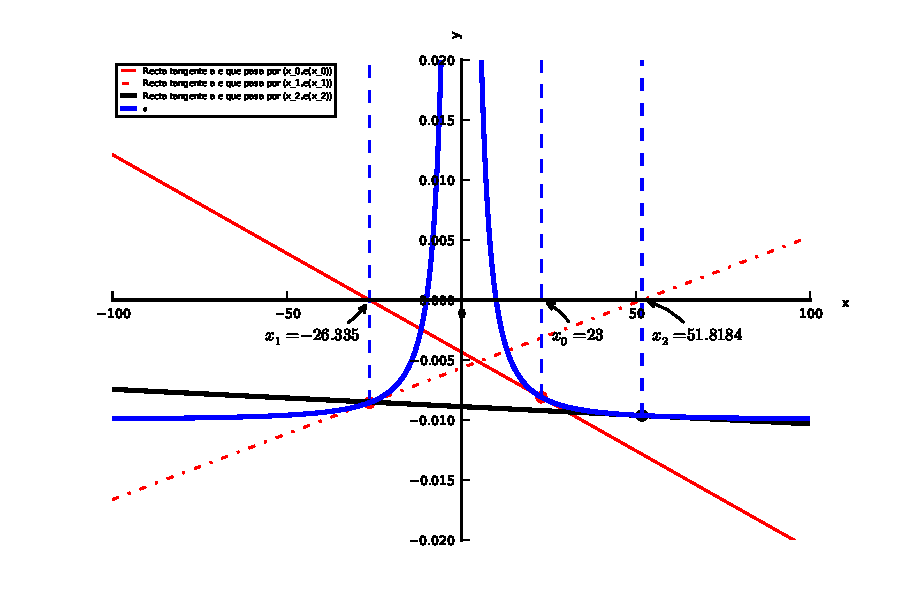
\includegraphics[keepaspectratio]{../Imagenes/exp1/divergencia.pdf}
		  \caption{Rectas tangentes a la función e con $\alpha=0.01, \frac{1}{\sqrt{\alpha}} = 10$ en $x_0= 23, x_1= -26.335, x_2=51.8184$ (primeras 3 iteraciones)}
		  \label{fig:contra1}
	\end{center}
\end{figure}
\FloatBarrier

Este gráfico nos da una idea de la causa de la divergencia para determinados valores iniciales mayores a los de la raíz buscada. La pendiente de la recta tangente en un punto está determinada por la función
e\_derivada: $\frac{-2}{x^{3}}$. Notemos que, luego de la primera iteración el valor obtenido es -26.335 $\Rightarrow$ el módulo de la pendiente de la recta tangente que pasa por $(x_1,e(x_1))$ es menor que
el anterior. Como consecuencia, la intersección de esta recta con el eje x se produce en x=51.8184, valor considerablemente más alejado del 0 que el $x_0$ inicial. De esta manera, sucesivas iteraciones 
generan puntos más distantes al 0, por lo que las pendientes de las rectas tangentes se vuelven cada vez menores en módulo, generando un círculo vicioso en donde el método diverge. Observemos cono la recta
tangente correspondiente a $(x_2,e(x_2))$, de color negro, no llega a cortar al eje x debido a su peque\~na pendiente. De hecho, esto ocurre recién en x = -617.971.

Al estudiar la convergencia de Secante\_f obtuvimos resultados bastante similares a los de Newton\_f. Empíricamente, el método converge para cualquier par de valores iniciales. Los experimentos
fueron probados para valores de $\alpha \in (0,1] \cup [1,20] \cup [1000,1010] \cup [10^{6},10^{6}+10]$, probando por cada valor distintos pares de semillas iniciales. Por ejemplo, con valores
$x_0,x_1 \in (0,1]$, $x_0 \in (0,1] \ \wedge \ x_1 \in (1,20]$, $x_0 \in (0,1] \ \wedge \ x_1 \in [1000,1010]$ , etc.

Estudiemos momentáneamente la estructura de cada iteración:

$x_{n+1} = x_n - \frac{(x_n-x_{n-1})*f(x_n)}{f(x_n)-f(x_{n-1})}$

De la fórmula se deduce que, si en algún momento $x_n = x_{n-1}$ entonces el método puede llegar a comportarse de una forma indeseada (Se realiza una división por cero, o un valor muy cercano a cero).
Por este motivo, debemos cuidarnos fundamentalmente de 2 aspectos:

a- No comenzar a iterar con semillas iniciales tales que $x_0 = x_1$.

b- Parar las iteraciones cuando $x_n \approx x_{n-1}$. En el caso de utilizar malos criterios de parada, como por ejemplo el 1: i = max\_iter
lo que sucede es que el método encuentra la raíz buscada y luego diverge, debido a que intenta continuar realizando las iteraciones.

Con Secante\_e también obtuvimos resultados similares a los de Newton\_e. El método converge con seguridad cuando $x_0,x_1 \in (0,\frac{1}{\sqrt{\alpha}}]$ Si una de las 2 semillas es mucho mayor a la raíz, lo más
probable es que el método diverja, ya que las rectas tangentes se comportan de forma muy parecida a las secantes.

~

Finalmente, para cerrar con esta primera parte, a la cual llamamos \underline{Primeras experimentaciones}, incluímos tres gráficos correspondientes a Bisección\_e, Secante\_e y Newton\_e, con el objetivo de
visualizar de forma más clara la forma en la que los métodos convergen a la raíz teórica en función de la cantidad de iteraciones. Todos ellos fueron graficados en función de los mismos datos: $\alpha = 0.01$,
criterio de parada 2 y un error $\epsilon=10^{-8}$

\begin{figure}[!h]
	\begin{center}
		  \includegraphics[keepaspectratio]{../Imagenes/exp2/biseccion_e.pdf}
		  \caption{Método de bisección\_e con los parámetros anteriormente mencionados, y semillas iniciales: $x_0 = 100, x_1=\alpha=0.01$}
		  \label{fig:contra1}
	\end{center}
\end{figure}
\FloatBarrier

Si bien en la figura anterior el método comienza con semillas bastante separadas (100 unidades aproximadamente), luego de la cuarta iteración la distancia entre ambas es solamente de 6 unidades, por lo que
alcanza el punto en donde comienzan los otros métodos. Sin embargo, realiza 30 iteraciones y aún así no llega a encontrar un resultado con un error menor al exigido: $10^{-8}$

\begin{figure}[!h]
	\begin{center}
		  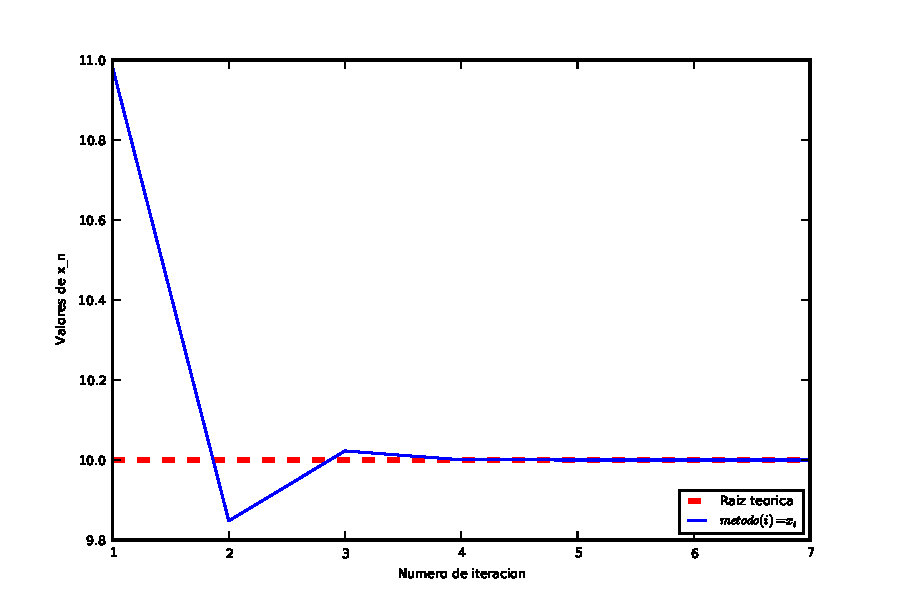
\includegraphics[keepaspectratio]{../Imagenes/exp2/secante_e.pdf}
		  \caption{Método de secante\_e con los parámetros anteriormente mencionados, y semillas iniciales: $x_0=1, x_1=11$ }
		  \label{fig:contra1}
	\end{center}
\end{figure}
\FloatBarrier

El criterio de parada se alcanza luego de la 7ma iteración en este experimento de secante\_e.

\begin{figure}[!h]
	\begin{center}
		  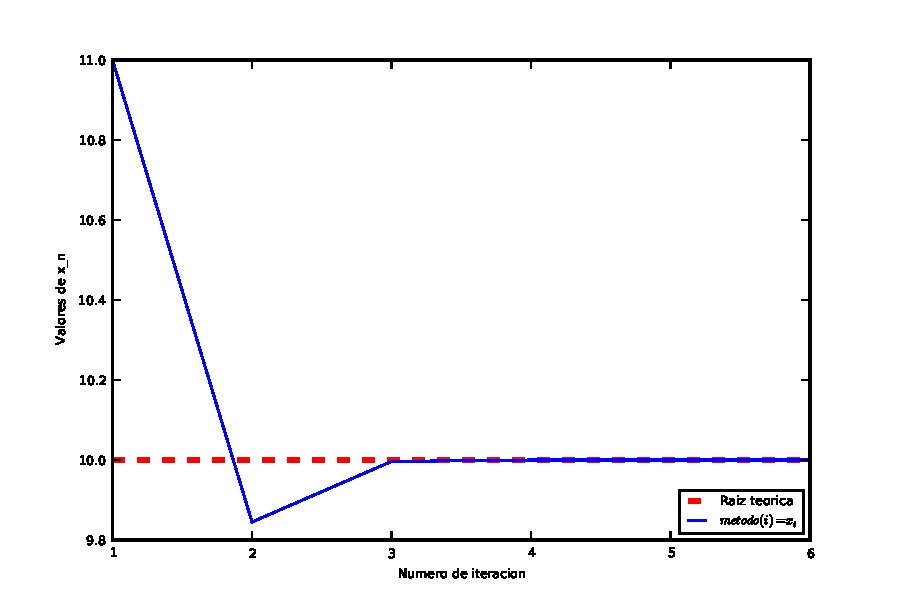
\includegraphics[keepaspectratio]{../Imagenes/exp2/newton_e.pdf}
		  \caption{Método de newton\_e con los parámetros anteriormente mencionados, y semilla inicial: $x_0=11$}
		  \label{fig:contra1}
	\end{center}
\end{figure}
\FloatBarrier

El criterio de parada se alcanza luego de la 6ta iteración en este experimento de Newton\_e.

\begin{figure}[!h]
	\begin{center}
		  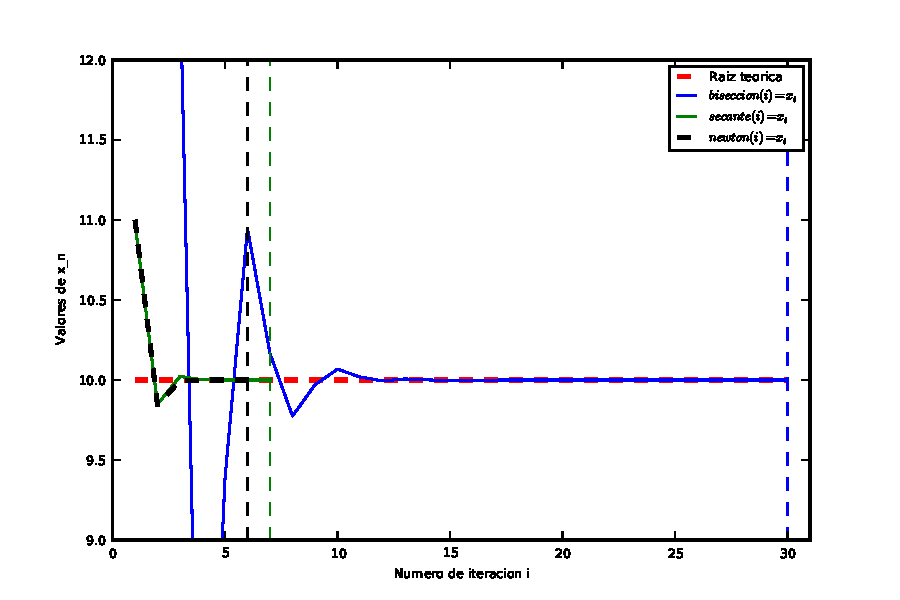
\includegraphics[keepaspectratio]{../Imagenes/exp2/todos_juntos.pdf}
		  \caption{Todos juntos en un mismo gráfico}
		  \label{fig:contra1}
	\end{center}
\end{figure}
\FloatBarrier

\section{Discusión}

 


\section{Conclusiones}

El trabajo nos permitió estudiar y analizar empíricamente el comportamiento los algoritmos iterativos aprendidos en clase que sirven para hallar raíces de funciones reales ($R \rightarrow R$).

Tal como mencionamos en el desarrollo, una porción muy grande de la experimentación estuvo enfocada en comprobar si los métodos convergían o no a la solución, y en caso de no hacerlo, intentar explicar las
causas de dicho comportamiento. Efectivamente, los 3 algoritmos implementados (para ambas funciones) convergen a las raíces. Si bien es cierto que en esta primera etapa de la experimentación $Secante\_e$ y
$Newton\_e$ divergieron para ciertos valores de $\alpha$ y semillas iniciales , esto no entró en contradicción con la teoría sino todo lo contrario.
Los teoremas de convergencia de Newton y Secante nos hablan de un entorno alrededor de la raíz sobre el cual no tenemos ningún tipo de control. Al probar nuevamente los métodos utilizando los mismos valores 
de $\alpha$ que anteriormente habían fallado, pero esta vez con valores iniciales más cercanos a las soluciones los métodos convergieron.

Una vez asegurado el aspecto más importante de los algoritmos pudimos hilar un poco más fino y concentrarnos en otro tipo de aspectos. Determinar un buen criterio de parada resulta importante para encontrar un
balance entre tiempo de ejecución (reflejado en la cantidad de iteraciones que tiene que hacer cada método) y calidad de la solución obtenida (orden de magnitud del error entre la solución obtenida y la
solución teórica). Con un criterio muy restrictivo los métodos podrían realizar una cantidad de iteraciones innecesaria. Con uno muy laxo podríamos llegar a una solución muy poco precisa. Luego de la 
experimentación llegamos a la conclusión de que los criterios 4 y 5 (relacionados con la imagen de los valores de la sucesión) funcionan aceptablemente con la función $f$, mientras que los criterios 2 y 3
(relacionados con los valores de la sucesión) se adapta mejor a la función $e$. El criterio 6 es el más restrictivo de todos y empíricamente registra un mal comportamiento, ya que realiza un cociente con 
un divisor que cada vez es más cercano a 0 a medida que el método converge.

En cuanto al problema de la semilla inicial y el número de iteraciones de bisección para el hallazgo de una buena semilla, vimos que combinar bisección con otro método es una buena solución que hace más eficiente el resultado. Definir cuántas iteraciones hacer es más delicado y en muchos casos depende del $\alpha$ en cuestión. 
Llegamos a la conclusión de que sobre $f(x)$, independientemente de cual sea el valor de $\alpha$ unas pocas iteraciones de bisección bastan y como planteamos en la hipótesis creemos que 4-5-6 son suficientes.
Sobre $e(x)$ en cambio el valor de $\alpha$ influye mucho más por lo que una cantidad de iteraciones variable puede ser la solución. Concluimos que con 5 a 9 iteraciones de bisección basta para alphas más o menos cercanos a 1 y aumentar la cantidad de iteraciones para valores de $\alpha$ más chicos o mucho más grandes, con valores entre las 15 y 25 iteraciones.

Al final de la experimentación analizamos los tiempos, y pudimos comprobar que la implementación de Newton efectivamente consume menor cantidad de ciclos de clock que los otros métodos, seguido de Secante 
y Bisección (en ese orden). Nuevamente, los resultados experimentales concuerdan con lo esperado a nivel teórico, ya que Newton tiene convergencia cuadrática, Secante tiene convergencia superlineal y Bisección
es lineal.

A nivel un poco más personal creemos que el trabajo resultó interesante y didáctico. Si bien el enunciado era muy claro nos dejaba una gran libertad a la hora de realizar y planificar la parte experimental,
por lo que fue importante ser creativos y al mismo tiempo claros acerca de los puntos sobre los cuales quisimos experimentar y cómo mostrar los resultados. Aprender a utilizar los graficadores y automatizar
los tests fue sin dudas un desafío muy grande que tuvimos que enfrentar en este trabajo.

\section{Apéndices}

\subsection{Apéndice A: Enunciado}

\parindent = 0 pt
\parskip = 11 pt

El objetivo del trabajo pr\'actico consiste en implementar un programa que permita calcular, dado $\alpha \in
\mathbb{R}$, $1/\sqrt{\alpha}$. Para ello, se deber\'a considerar las funciones $f(x)$ y $e(x)$ definidas
anteriormente, distintos m\'etodos vistos en clase que permitan resolver el problema planteado y realizar un an\'alisis
completo del comportamiento de los mismos. 

Los requisitos m\'inimos a cumplir son los siguientes:

\begin{itemize}
\item Implementar el m\'etodo de Newton para la funci\'on $f(x)$. Incluir en el informe la demostraci\'on de
convergencia (Ejercicio 3, Pr\'actica 1). Para la funci\'on $e(x)$, implementar al menos dos m\'etodos (uno de los
cuales debe ser el de Newton).   
\item Para cada m\'etodo, estudiar experimentalmente la convergencia, tiempo de ejecuci\'on, cantidad de iteraciones,
criterios de parada, precisi\'on en el resultado, y cualquier otro par\'ametro que considere necesario evaluar. Realizar experimentos
computacionales considerando un rango amplio de valores posibles para $\alpha$ y distintos puntos iniciales
para los m\'etodos. Analizar y justificar detalladamente los resultados obtenidos.
\item Una vez fijados los mejores par\'ametros para cada m\'etodo, realizar una comparaci\'on entre las tres formas
alternativas de resolver el problema (Newton para $f(x)$, y Newton m\'as el otro m\'etodo para $e(x)$) en t\'erminos de
tiempo de ejecuci\'on, precisi\'on en la soluci\'on, cantidad de iteraciones, etc. Determinar experimentalmente que
variante seleccionar\'ia para su utilizaci\'on en la pr\'actica.
\end{itemize}

\subsection{Apéndice B: Código}

Los métodos reciben un booleano como parámetro: $hacerBiseccion$. Si el valor del mismo es 1, entonces realiza previamente
$cantItBis$ iteraciones de bisección y comienza con esos valores iniciales. De lo contrario, utiliza como semillas las que
recibe como parámetro.

M\'etodo de Bisección para la funci\'on $f(x)$:

\lstset{caption=Biseccion, label=b; framexleftmargin=2mm, frame=shadowbox, rulesepcolor=\color{black}, language={[ANSI]C}}
\tiny{
\lstinputlisting[language=C++]{codigo/biseccion.cpp}
}

\normalsize{M\'etodo de Newton para la funci\'on $f(x)$:}

\lstset{caption=Newton,label=Newt, framexleftmargin=2mm, frame=shadowbox, rulesepcolor=\color{black}, language={[ANSI]C}}
\tiny{\lstinputlisting[language=C++]{codigo/newton.cpp}}

\normalsize
(*) $x_{n+1} = x_{n} - \frac{f(x_{n})}{f'(x_{n})}$

M\'etodo de Secante para la funci\'on $f(x)$:

\lstset{caption=Secante,label=Sec, framexleftmargin=2mm, frame=shadowbox, rulesepcolor=\color{black}, language={[ANSI]C}}
\tiny{
\lstinputlisting[language=C++]{codigo/secante.cpp}
}

\normalsize
(**) $x_{n+1} = x_{n} - \frac{f(x_{n})*(x_{n}-x_{n-1})}{f(x_{n})-f(x_{n-1})}$

No se incluyen los c\'odigos para la funci\'on $e(x)$ ya que son exactamente id\'enticos, cambiando $f(x)$ y $f\_deriv(x)$ por $e(x)$ y $e\_deriv(x)$ respectivamente.

\lstset{caption=Semillas iniciales,label=Sem, framexleftmargin=2mm, frame=shadowbox, rulesepcolor=\color{black}, language={[ANSI]C}}
\tiny{
\lstinputlisting[language=C++]{codigo/seeds_iniciales.cpp}
}

\normalsize

\underline{\emph{Semillas iniciales}}

\underline{\emph{f:}} (*)

\begin{algorithmic} 
	\If{$\alpha < 1$} 
		\State $semilla\_positiva = 1$
		\State $semilla\_negativa = \alpha$
	\Else
		\State $semilla\_positiva = \alpha$
		\State $semilla\_negativa = 1$
	\EndIf
\end{algorithmic}

~

\underline{\emph{e:}} (**)

\begin{algorithmic} 
	\If{$\alpha < 1$} 
		\State $semilla\_positiva = \alpha$
		\State $semilla\_negativa = \frac{1}{\alpha}$
	\Else
		\State $semilla\_positiva = \frac{1}{\alpha}$
		\State $semilla\_negativa = \alpha$
	\EndIf
\end{algorithmic}

\subsection{Apéndice C: Criterios de parada}

1) $n = MAX\_ITER$

2) $|x_{n} - x_{n-1}| < \epsilon$

3) $\frac{|x_{n} - x_{n-1}|}{|x_{n-1}|} < \epsilon$

4) $|f(x_{n})| < \epsilon$

5) $|f(x_{n})-f(x_{n-1})| < \epsilon$

6) $\frac{|f(x_{n}) - f(x_{n-1})|}{|f(x_{n-1})|} < \epsilon$

\vspace{2cm}

\subsection{Apéndice D: Demostración}
Secante
Sea $f(x) = x^2 -a$ una funci\'on a la cual se le quiere encontrar raices.Para ello se propone una sucesi\'on de punto fijo $x_{n+1} = g(x_n) = \frac{1}{2}\left(x_n+ \frac{a}{x_n}\right)$. Veamos si efectivamente $g(x)$ corresponde con el m\'etodo de Newton.

Sea $f(x) = x^2 - a$ $\Rightarrow$ $f'(x) = 2x$. Por lo tanto, la sucesi\'on del m\'etodo de Newton es la siguiente: $g_{2}(x_n) = x_n - \frac{(x_{n}^2 -a)}{2x_n}$. 

Queremos ver que $g_2(x_n)=g(x_n)$ 

$\displaystyle g_{2}(x_n) = \displaystyle x_n - \frac{(x_{n}^2 -a)}{2x_n}$ $=$ $\displaystyle \frac{1}{2}\left(2x_n - \frac{x_{n}^2 - a}{x_n}\right)$ $=$ $\displaystyle \frac{1}{2}\left(\frac{2x_{n}^2 -x_{n}^2 + a}{x_n}\right) = \frac{1}{2}\left(\frac{x_{n}^2 + a}{x_n}\right) = \frac{1}{2}\left(x_{n} + \frac{a}{x_n}\right) = g(x_n)$

Luego hay que probar que si $x_0 > \sqrt{a}$ entonces $x_{n+1} < x_n$ para $n \geq 0$.

Ant\'es que nada probemos una propiedad que vamos a utilizar m\'as adelante:

\hspace{6.5cm}$x_0 > \sqrt{a} \Rightarrow x_n > \sqrt{a}$ (P1). 

Mediante inducci\'on, definimos el esquema inductivo a probSecantear como:

Sea $P_1(n):=$ $x_0 > \sqrt{a} \Rightarrow x_n > \sqrt{a} $
\begin{itemize}
	\item Caso base: $P_1(0) \land P_1(1)$ 
	\item Caso inductivo: $P_1(n) \Rightarrow P_1(n+1)$
\end{itemize}

Probar $P_1(0)$ es trivial porque es exactamente el lado izquierdo de la implicaci\'on. Veamos $P_1(1)$

\hspace{4cm}$\displaystyle  x_1 > \sqrt{a} \equiv g(x_0) > \sqrt{a} \equiv \frac{1}{2}\left(x_0+ \frac{a}{x_0}\right) > \sqrt{a} \equiv x_0+ \frac{a}{x_0} > 2\sqrt{a}\equiv$


\hspace{4cm}$\displaystyle  x_{0}^2+ a > 2x_{0}\sqrt{a}$ \footnotemark[1] $\equiv$	$x_{0}^2 - 2x_{0}\sqrt{a} + a > 0$ $\equiv$ $\left(x_{0} - \sqrt{a}\right)^2 > 0$

1: Como $x_0 > \sqrt{a} > 0$ entonces la desigualdad no cambia de sentido.

Como $x_0 > \sqrt{a}$ entonces vale que $\left(x_{0} - \sqrt{a}\right)^2 > 0$.

Luego, para el caso inductivo se procede de la misma forma que en el caso base, pero intercambiando $x_1$ por $x_{n+1}$ y $x_0$ por $x_n$, de modo que queda:

\hspace{4cm}$\displaystyle  x_{n+1} > \sqrt{a} \equiv g(x_n) > \sqrt{a} \equiv \frac{1}{2}\left(x_n+ \frac{a}{x_n}\right) > \sqrt{a} \equiv x_n+ \frac{a}{x_n} > 2\sqrt{a}\equiv$


\hspace{4cm}$\displaystyle  x_{n}^2+ a > 2x_{n}\sqrt{a}$ \footnotemark[2] $\equiv$	$x_{n}^2 - 2x_{n}\sqrt{a} + a > 0$ $\equiv$ $\left(x_{n} - \sqrt{a}\right)^2 > 0$


2: Como $x_n > \sqrt{a} > 0$ entonces la desigualdad no cambia de sentido.

Y nuevamente, como $x_n > \sqrt{a}$, entonces vale que $\left(x_{n} - \sqrt{a}\right)^2 > 0$.

Lo interesante de la propiedad (P1) es que nos permite implicar que $(\forall n \geq 0) x_n > 0$.

Ahora, volviendo al problema original.

Sea $P(n):=$ $x_0 > \sqrt{a} \Rightarrow x_{n+1} < x_{n}$
\begin{itemize}
	\item Caso base: $P(0) = x_0 > \sqrt{a} \Rightarrow x_1 < x_0$
	\item Caso inductivo: $((\forall n\geq 0)$ $P(n)) \Rightarrow P(n+1)$
\end{itemize}

Caso base:


\hspace{4cm}$\displaystyle x_1 < x_0 \equiv g(x_0) < x_0 \equiv \frac{1}{2}\left(x_0 + \frac{a}{x_0}\right) < x_0 \equiv \left(x_0 + \frac{a}{x_0}\right) < 2x_0 \equiv$


\hspace{4.5cm}$\displaystyle \frac{a}{x_0} < x_0 \equiv a < x_{0}^2$ $\Rightarrow \sqrt{a} < |x_0| \equiv \sqrt{a} < x_0 \equiv P(0)$

Caso inductivo:
 
\hspace{4cm}$\displaystyle  x_{n+2} < x_{n+1} \equiv g(x_{n+1}) < x_{n+1} \equiv \frac{1}{2}\left(x_{n+1} + \frac{a}{x_{n+1}}\right) < x_{n+1} \equiv $


\hspace{4cm}$\displaystyle  \left(x_{n+1} + \frac{a}{x_{n+1}}\right) < 2x_{n+1} \equiv \frac{a}{x_{n+1}} < x_{n+1} \equiv a < x_{n+1}^2 \equiv $


\hspace{4cm}$\displaystyle  \sqrt{a} < |x_{n+1}| \equiv \sqrt{a} < x_{n+1} <\footnotemark[3]$  $x_n < \ldots < x_0 \Rightarrow \sqrt{a} < x_0$


3: Por hip\'otesis inductiva.


\section{Referencias}

\begin{itemize}
	\item $^1$ http://math.fullerton.edu/mathews/n2003/FixedPointMod.html para más información, 

	y unas animaciones didácticas: 

	http://math.fullerton.edu/mathews/a2001/Animations/RootFinding/FixedPoint/FixedPoint.html
	\item $^2$ http://nm.mathforcollege.com/topics/newton$\_$raphson.html
	\item $^3$ http://nm.mathforcollege.com/topics/bisection$\_$method.html
	\item $^4$ http://nm.mathforcollege.com/topics/secant$\_$method.html $\&$ 

	http://nm.mathforcollege.com/topics/false$\_$position.html
\end{itemize}


\end{document}
